\documentclass[12pt]{article}
\usepackage{graphicx} % Required for inserting images
\usepackage{tikz}
\usetikzlibrary{external}
\tikzexternalize[prefix=tikz/]
\usepackage{placeins}
\usepackage[utf8]{inputenc}
\usepackage{placeins}
\usepackage{setspace}
\usepackage[backend = biber, style= mla]{biblatex}
\usepackage{csquotes}
\setstretch{1.5}
\usepackage{multicol}
\bibliography{refs}
\RequirePackage{newfloat} %% For placing figures in the right place
\usepackage{fancyhdr} %% For custom headers and footers
\usepackage{caption} %% For custom captions
\usepackage[top=1in,bottom=1in,left=0.75in,right=0.75in]{geometry} 
\usepackage{array}
\usepackage[T1]{fontenc}
\usepackage[english]{babel}
\usepackage{graphicx}
\usepackage{appendix}
\usepackage[siunitx, EFvoltages]{circuitikz}
\usepackage{siunitx}
\usepackage{booktabs}
\usepackage{subcaption}
\usepackage{multirow}
\usepackage{float}
\usepackage{physics}
\usepackage{makecell}
\usepackage[makeroom]{cancel}
\usepackage{enumerate}
\usepackage{hyperref}
    \hypersetup{
    colorlinks=true,
    breaklinks=true,
    citecolor=blue,
    linkcolor=black,
    urlcolor=blue,
    }
\numberwithin{equation}{section}
\usepackage[nottoc, notlot, notlof, numbib]{tocbibind}
\usepackage[labelfont=bf]{caption}
\usepackage{amsfonts,amsmath,amssymb}
\usepackage{fancyhdr} %Fancy Title 
\usepackage{setspace}
\usepackage{array}
    \newcolumntype{P}[1]{>{\centering\arraybackslash}p{#1}}
    \newcolumntype{M}[1]{>{\centering\arraybackslash}m{#1}}
\usepackage{multirow}
\usepackage{blindtext}
\usepackage{listings}
\usepackage{pgfplots}
\usepackage[siunitx]{circuitikz} %[symbols]
\usepackage[outline]{contour} % glow around text
\usetikzlibrary{arrows,arrows.meta}
\usetikzlibrary{decorations.markings}
\tikzset{>=latex} % for LaTeX arrow head
\usepackage{xcolor}
\colorlet{Icol}{blue!50!black}
\colorlet{Ccol}{orange!90!black}
\colorlet{Rcol}{green!50!black}
\colorlet{loopcol}{red!90!black!25}
\colorlet{pluscol}{red!60!black}
\colorlet{minuscol}{blue!60!black}
\newcommand\EMF{\mathcal{E}} %\varepsilon}
\contourlength{1.5pt}
\tikzstyle{EMF}=[battery1,l=$\EMF$, invert]
\tikzstyle{internal R}=[R,color=Rcol,Rcol,l=$r$,/tikz/circuitikz/bipoles/length=30pt]
\tikzstyle{loop}=[->,red!90!black!25]
\tikzstyle{loop label}=[loopcol,fill=white,scale=0.8,inner sep=1]
\tikzstyle{thick R}=[R,color=Rcol,thick,Rcol,l=$R$]
\tikzstyle{thick C}=[C,thick,color=Ccol,Ccol,l=$C$]
\tikzstyle{myswitch}=[closing switch,line width=0.3] %-{Latex[length=3]},
\DeclareMathOperator\arctanh{arctanh}
\newcommand{\myvoltmeter}[2] 
{  % #1 = name , #2 = rotation angle
  \begin{scope}[transform shape,rotate=#2]
  \draw[thick] (#1)node(){$\mathbf V$} circle (11pt);
  \draw[rotate=45,-latex] (#1)  +(-17pt,0) --+(17pt,0);
  \end{scope}
}
\ctikzset{bipoles/thickness=1.2}
\newcommand{\midlabelline}[3]{
   \node (midlabel) at ($ (#1)!.5!(#2) $) {#3};
   \draw[latex-] (#1) --  (midlabel);
   \draw[-latex] (midlabel) -- (#2);
}

\renewrobustcmd{\footcite}[1]{
    \footfullcite{#1}
}


\floatplacement{graph}{H} %% Graphs are placed in the right place


\makeatletter
\renewcommand{\@floatboxreset} {%
        \reset@font
        \normalsize
        \@setminipage
\centering%<<<<<<<<<<<<<<<<<<<
}
\makeatletter

\DeclareFloatingEnvironment{graph}




%% Table of contents options
\renewrobustcmd{\tableofcontents}{
    \pagestyle{empty}
    \section*{Table of Contents}
    \vspace*{0.5cm}
    \hrule
    \vspace*{0.5cm}
    \@starttoc{toc}
    \newpage
    \setcounter{page}{1}
    \pagestyle{fancy}
    \restoregeometry
}

\NeedsTeXFormat{LaTeX2e}
\ProvidesPackage{main}[2023/05/23 baskerville's Package]
%%Package options
%% This loads all the requiered packages for a proper compilation. However
%% future versions may affect the processing of the document. Therefore, it
%% TODO add version dates to all packages
%% TODO add warnings for outdated packages
\RequirePackage{etoolbox} %% Control sequence commands
\RequirePackage{lipsum} %% Lorem ipsum generator
\RequirePackage{ragged2e} %% For justifying text in Math IA's
\RequirePackage{lastpage} %% For retriving the total number of pages in the
%% typsset document
\babelprovide[import,main]{english} %% Main language
\justifying %% This is a must for Math IA's, and is loaded from the ragged2e:
%% https://ctan.org/pkg/ragged2e?lang=en.

\fancyhead[C]{\small\scshape\@title} %% The title of the document is placed
%% in the center of the header. This is completly optional, and can be removed.
\fancyhead[R]{\small\scshape{\thepage/\pageref{LastPage}}} %% The page number
%% along with the total number of pages is placed in the right side of the
%% footer. This isnt required, but is an asthetic choice.
\fancyfoot{\hrule}
\addbibresource{mla.bib}  
\title{IB Physics HL Internal Assessment}
\date{\vspace{-2.85cm}}
\begin{document}
\maketitle
{\LARGE{How Does the Temperature of Distilled Water Affect the Capacitance of 3 Submerged Capacitors Connected in Series?}}
\section{Introduction}
\noindent It is well-established that leaving an electronic device, most popularly a cell phone, in an extremely cold or hot environment can harm its battery life and longevity, even diminishing the central processing unit's (CPU) performance. While I usually keep my cell phone dry and at reasonable temperatures, some family members use theirs for music in the shower or swimming. While newer phones are water resistant and the central battery is rarely affected by this exposure, many of my relatives mention a pronounced decrease in battery life and charging times for their cell phones. At the same time, I had not experienced anything similar. Some components of the phone are affected by temperature and water vapor besides the battery. Upon researching phone components, I came across the culprit: capacitors. Phones use hundreds of capacitors to regulate the charging and discharging of every component. However, the focus is often placed on the battery, and many of the reductions in phone performance are attributed to "natural wear" and "software aging." This exploration focuses on observing the changes that a capacitor undergoes when subject to such temperature changes, specifically when submerged in water, the most common substance found in infiltrating electronic systems.\\
\noindent This Internal Assessment will explore the research question: How does the temperature of distilled water affect the capacitance of submerged 3 capacitors connected in series? 

\section{Theory}
\noindent Capacitors aid batteries within electronics discharge and power-specific components at specific times. While a phone powered solely by a capacitor would only stay powered for minutes, using them with chemically powered batteries allows for a much more efficient system. Particularly, capacitors significantly affect cell phones' charging speed, and any hindrance to their function can cause lapses in charging times. Regarding my aforementioned anecdote, there is evidence of some impact of temperature on the ability of a capacitor to discharge and hold charge. Furthermore, the presence of water vapor - more likely condensed water once the steam has entered a phone - seems to detrimentally affect the charging speed of the battery\footfullcite{capacitorsinsmartphoneantennasystems2022}. To understand why this might be, capacitors must be understood on a particulate level. The capacitance $C$ of a capacitor quantifies its ability to store charge. For a traditional parallel plate capacitor \footfullcite{capacitor_schematic_with_dielectric}
\begin{equation}
    C = \frac{\kappa \epsilon_0 A}{d}
\end{equation}
Where $\kappa$ is the dielectric constant, $\epsilon_0$ is the permittivity of free space, $A$ is the surface area of either capacitor plate, and $d$ is the distance between the capacitors. In the case of a submerged capacitor, the dielectric is water, which normally has a constant dielectric value but with varying temperature changes. Like more traditional dielectrics, the water molecules within the dielectric (ignoring edge effects) will align along the capacitor's imposed electric field, leading to an opposing electric field. In the case of a polar water molecule, the positively charged dipole near the hydrogen atoms will be located farther along the electric field. In contrast, the negatively charged dipole near the oxygen atoms will be located farther opposite the electric field. Specifically, the negative and positive dipoles will face the opposing charge on each capacitor plate.\\
\noindent However, as temperature changes, the ability of water molecules to oppose the capacitor's electric field changes. At higher temperatures, the Brownian motion of the water molecules should lead to such rapid motion that a proper alignment mechanism of the molecules will not have enough time to occur, and on average, they will not opposite the electric field. At lower temperatures, however, the capacitance should increase due to the increasingly static motion of the water molecules throughout the volume, which allows the individual molecules to be oriented by the electric field \footfullcite{physicsforums_capacitor_charge}. 
3 series capacitors have been chosen for this model to reflect the charging system of my phone. Though my phone has far more capacitors, the model is the closest recreation I can produce with the available resources.


\section{Methodology}
\subsection{Variables}
The \textbf{independent variable} in this experiment is the temperature of the water surrounding the circuit. The \textbf{dependent variable} is the capacitance of each submerged capacitor. The \textbf{controlled variables} are the volume of water, the type of capacitor used, the setup of the circuit (3 capacitors in series connected to an emf), the voltage of the battery, and adjusting time, which was about 5 minutes after each temperature increase given to the capacitors to adjust and stabilize. All circuit components remained identical throughout the experiment. A diagram of the experiment is shown below\footnote{Cn refers to the nth capacitor}:

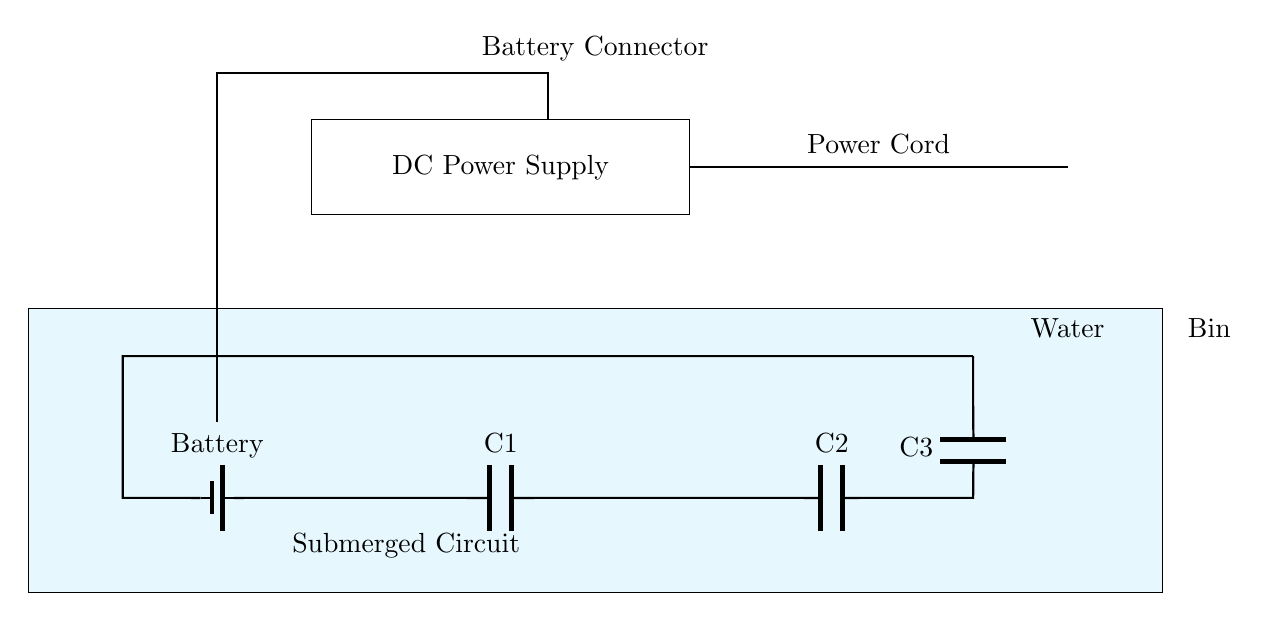
\begin{tikzpicture}[scale=1.2]
    % Draw the bin of water
    \filldraw[fill=cyan!10, draw=black] (-1, -2) rectangle (11, 1);
    \node at (10,0.8) {Water};
    \node at (11.5, 0.8) {Bin};
    % Draw the DC power supply outside the bin
    \draw (2,2) rectangle (6, 3) node[pos=.5] {DC Power Supply}; % Power supply to battery connection

    % Draw the submerged circuit
    \draw[thick]
    (0,0) -- (0,-1) % Line from battery to submerged
    to[battery1, l=Battery] (2,-1)
    to[C, l=C1] (6,-1)
    to[C, l=C2] (9,-1)
    to[C, l=C3] (9,0) -- (9,0.5) % Return to above water
    (9,0.5) -- (0,0.5) -- (0,0.5) -- (0,-1);% Closing the circuit loop
    
    % Label the submerged circuit
    \node[align=center] at (3,-1.5) {Submerged Circuit};

    % Draw the power cord
    \draw[thick] (1, -0.2) -- (1, 3.5) -- (4.5, 3.5)--(4.5,3); % Power supply cord
    \node[align=center] at (5, 3.75) {Battery Connector};

    \draw[thick] (6, 2.5) -- (10,2.5); % 
    \node[align=center] at (8, 2.75) {Power Cord};
\end{tikzpicture}


\subsection{Apparatus}
The volume of the insulating container was chosen as 0.1L to match my phone's volume, to minimize the deviation caused by a larger body of water and movement. 

\begin{spacing}{1.14}

\begin{itemize}
    \item 3 Identical Commercial Capacitors of Known Capacitance
    \item At least 2.5 Liters of Distilled Water
    \item 0.1 Litres Volume Insulating Container
    \item Temperature-controlled water bath; VWR WB02 2L Digital Water Bath (capable of holding a 0.1 litre container)
    \item 1x Vernier LabQuest 2
    \item 1x Tenma 72-8150 Capacitance Meter
    \item 0.05m of insulated wire of known resistivity (preferably extremely low)
    \item 3.85 Volts Waterproof Insulated Battery with a Direct Current Power Supply
    \item 2 oz J-B Weld Epoxy Putty Waterproof Adhesive with 1x Liouhoum Soldering Iron Kit
    \item 1x Wastebin (preferably with volume 5 Litres or above)
\end{itemize}

\subsection{Procedure}
\begin{enumerate}
    \item Assemble the series circuit with the 3 capacitors in series and the battery, linked by insulating wire all soldered together.
    \item Place the circuit in the insulating container and secure each component to the bottom with waterproof adhesive. Connect the circuit to the power supply.
    \item Using the water bath, heat the 0.1 Litres of water to the desired temperature. Pour this water into the insulating container gently until full, and close the container.
    \item Allow 5 minutes and then measure the capacitance of each capacitor using the Capacitance Meter. Wait 10-15 seconds for the values to stabilize. Ensure no significant changes in temperature with the LabQuest, and if there are, the trial must be repeated.
    \item Once measurements have finished, carefully empty the water from the container into the wastebin, and repeat for all desired temperature values.
\end{enumerate}
\end{spacing}
\subsection{Challenges and Ethics}
After the first trial with room temperature water, I realized the difficulty in emptying the insulating water container. I decided to add waterproof adhesive to secure the circuit so that I could easily empty the container by flipping it upside down. Also, I originally did not consider some human error based on how quickly I closed the lid could lead to significant temperature changes, so I used the Vernier LabQuest to validate each trial and double-check the temperature of the water after the water bath as it had higher instrumental precision. 
\\
\noindent Regarding safety and environmental concerns, this experiment posed significanty necessity about care due to the use of electricity within water. Though distilled water was chosen, it likely would gain ions and become conductive over repeated trials, which prompted the use of new distilled water samples after each temperature increment, leading to 25 samples over 5 trials. Furthermore, an especially low current source was used, about 0.04 amps to avoid current damage to people or objects that came in contact - which was already minimized by the large insulating container where the experiment occurred. Gloves, safety goggles, and appropriate clothing were worn, and the experiment took place in an empty room devoid of any flammable or electronic devices due to the high-temperature water. The repeated usage of new water samples could be considered environmentally taxing, but the tiny sample size due to the small container size reduced the impact to a negligible level. Furthermore, the water bath chosen (VWR WB02 2L Digital Water Bath) was low-energy and efficient compared to other choices, minimizing energy consumption. All water, once used, was reused for gardening.

\section{Data}
The instrumental uncertainty for the LabQuest Mini was ($\pm 0.01 \, ^0 C$), and the Capacitance Meter was ($\pm 0.01 \, \mu F$), as both were digital and thus the uncertainty would be the smallest possible increment. C1 - C3 refers to capacitors 1-3, and T represents temperature (Capacitance for C1, C2, C3 vs Temperature Trials 1-5).
\subsection{Raw Data}
\vspace{0.5cm}
\FloatBarrier
\noindent
\begin{minipage}{0.5\textwidth}
    \centering
    \captionof{table}{Trial 1 Data}
    \begin{tabular}{@{}cccc@{}}
    \toprule
    T (°C) & C1 (µF) & C2 (µF) & C3 (µF) \\ \midrule
    20.00               & 2.87             & 2.89             & 2.85             \\
    25.00               & 2.84             & 2.86             & 2.82             \\
    30.00               & 2.80             & 2.82             & 2.78             \\
    35.00               & 2.75             & 2.77             & 2.73             \\
    40.00               & 2.70             & 2.72             & 2.68             \\ \bottomrule
    \end{tabular}
\end{minipage}%
\begin{minipage}{0.5\textwidth}
    \centering
    \captionof{table}{Trial 2 Data}
    \begin{tabular}{@{}cccc@{}}
    \toprule
    T (°C) & C1 (µF) & C2 (µF) & C3 (µF) \\ \midrule
    20.00               & 2.88             & 2.90             & 2.86             \\
    25.00               & 2.85             & 2.87             & 2.83             \\
    30.00               & 2.81             & 2.83             & 2.79             \\
    35.00               & 2.76             & 2.78             & 2.74             \\
    40.00               & 2.71             & 2.73             & 2.69             \\ \bottomrule
    \end{tabular}
\end{minipage}
\vspace{1cm}\\
\noindent
\begin{minipage}{0.5\textwidth}
    \centering
    \captionof{table}{Trial 3 Data}
    \begin{tabular}{@{}cccc@{}}
    \toprule
    T (°C) & C1 (µF) & C2 (µF) & C3 (µF) \\ \midrule
    20.00               & 2.89             & 2.91             & 2.87             \\
    25.00               & 2.86             & 2.88             & 2.84             \\
    30.00               & 2.82             & 2.84             & 2.80             \\
    35.00               & 2.77             & 2.79             & 2.75             \\
    40.00               & 2.72             & 2.74             & 2.70             \\ \bottomrule
    \end{tabular}
\end{minipage}
\begin{minipage}{0.5\textwidth}
    \centering
    \captionof{table}{Trial 4 Data}
    \begin{tabular}{@{}cccc@{}}
    \toprule
    T (°C) & C1 (µF) & C2 (µF) & C3 (µF) \\ \midrule
    20.00               & 2.90             & 2.92             & 2.88             \\
    25.00               & 2.87             & 2.89             & 2.85             \\
    30.00               & 2.83             & 2.85             & 2.81             \\
    35.00               & 2.78             & 2.80             & 2.76             \\
    40.00               & 2.73             & 2.75             & 2.71             \\ \bottomrule
    \end{tabular}
\end{minipage}
\vspace{1cm}\\
% Third row with one table centered
\noindent
\begin{minipage}{\textwidth}
    \centering
    \captionof{table}{Trial 5 Data}
    \begin{tabular}{@{}cccc@{}}
    \toprule
    T (°C) & C1 (µF) & C2 (µF) & C3 (µF) \\ \midrule
    20.00               & 2.91             & 2.93             & 2.89             \\
    25.00               & 2.88             & 2.90             & 2.86             \\
    30.00               & 2.84             & 2.86             & 2.82             \\
    35.00               & 2.79             & 2.81             & 2.77             \\
    40.00               & 2.74             & 2.76             & 2.72             \\ \bottomrule
    \end{tabular}
\end{minipage}

\FloatBarrier
\subsection{Processed Data}
The following processed data used the averages from Trials 1-5 mentioned above, maintaining the previously stated instrumental uncertainty. The uncertainty for each value was calculated by dividing the range by 2. Horizontal error bars were omitted as they were too small to be seen.\\
\textbf{Sample calculation for Uncertainty:}
Given the capacitance values for Capacitor 1 at 40°C across five trials are: 2.70 µF, 2.71 µF, 2.72 µF, 2.73 µF, and 2.74 µF. The average capacitance (\(C_{avg}\)) is calculated as:
\[
C_{avg} = \frac{\sum C_i}{N} = \frac{2.70 + 2.71 + 2.72 + 2.73 + 2.74}{5} = 2.72 \, \text{µF}
\]
The uncertainty is calculated as half the range of the measurements plus the instrumental uncertainty (0.01 µF). The range is the difference between the maximum and minimum values:
\[
\text{Range} = \max(C_i) - \min(C_i) = 2.74 - 2.70 = 0.04 \, \text{µF}
\]

\noindent Therefore, the average capacitance of Capacitor 1 at 40°C is 2.72 µF with an uncertainty of 0.03 µF (including the instrumental uncertainty of 0.01).

\FloatBarrier
\begin{table}[h!]
\centering
\caption{Average Individual Capacitance vs Temperature}
\begin{tabular}{@{}ccccc@{}}
\toprule
Temperature (°C) & Capacitor 1 (µF)  & Capacitor 2 (µF)  & Capacitor 3 (µF) \\ \midrule
20.00 & $ 2.89\pm 0.03$ & $2.91 \pm 0.03 $  & $2.87 \pm 0.03$ \\
25.00 & $2.86 \pm 0.03$ & $2.88\pm 0.03 $ & $2.84\pm 0.03 $\\
30.00  & $2.82\pm 0.03$   & $2.84\pm 0.03$ & $2.80\pm 0.03$  \\
35.00 & $2.77\pm 0.03$   & $2.79\pm 0.03 $   & $2.75\pm 0.03 $  \\
40.00  & $2.72\pm 0.03 $ & $2.74 \pm 0.03 $  & $2.70\pm 0.03$                 \\ \bottomrule
\end{tabular}
\end{table}
\FloatBarrier
\begin{figure}[h!]
    \centering
\begin{tikzpicture}
\begin{axis}[
    title={Average Capacitance vs. Temperature},
    xlabel={Temperature (°C)},
    ylabel={Capacitance (µF)},
    xmin=15, xmax=45,
    ymin=2.65, ymax=2.95,
    xtick={20,25,30,35,40},
    ytick={2.65,2.7,2.75,2.8,2.85,2.9,2.95},
    legend pos=north east,
    ymajorgrids=true,
    grid style=dashed,
    error bars/.cd,
    y dir=both,
    y explicit,
]

% Capacitor 1
\addplot[
    color=blue,
    mark=square,
    error bars/.cd, 
    y dir=both, 
    y explicit,
    ] 
    coordinates {
    (20,2.89) +- (0,0.03)
    (25,2.86) +- (0,0.03)
    (30,2.82) +- (0,0.03)
    (35,2.77) +- (0,0.03)
    (40,2.72) +- (0,0.03)
    };
    \addlegendentry{Capacitor 1}

% Capacitor 2
\addplot[
    color=red,
    mark=o,
    error bars/.cd, 
    y dir=both, 
    y explicit,
    ] 
    coordinates {
    (20,2.91) +- (0,0.03)
    (25,2.88) +- (0,0.03)
    (30,2.84) +- (0,0.03)
    (35,2.79) +- (0,0.03)
    (40,2.74) +- (0,0.03)
    };
    \addlegendentry{Capacitor 2}

% Capacitor 3
\addplot[
    color=green,
    mark=triangle,
    error bars/.cd, 
    y dir=both, 
    y explicit,
    ] 
    coordinates {
    (20,2.87) +- (0,0.03)
    (25,2.84) +- (0,0.03)
    (30,2.80) +- (0,0.03)
    (35,2.75) +- (0,0.03)
    (40,2.70) +- (0,0.03)
    };
    \addlegendentry{Capacitor 3}

\end{axis}
\end{tikzpicture}
    \caption{Average Capacitance vs Temperature for Capacitors 1-3 (Avg of Trials 1-5)}
    \label{fig:enter-label}
\end{figure}


\noindent \textbf{Equivalent Capacitance Calculation:} \noindent For \textbf{Table 7}, the equivalent capacitance was calculated as follows. The average capacitances for Capacitors 1, 2, and 3 at 40°C are 2.72 µF, 2.74 µF, and 2.70 µF, respectively.
Substituting into the equivalent capacitance for capacitors in series yields:
\[
\frac{1}{C_{eq}} = \frac{1}{2.72} + \frac{1}{2.74} + \frac{1}{2.70} = 0.3655
\]
\[
C_{eq} = \frac{1}{0.3655} = 0.907 \, \text{µF}
\]
\noindent Given the average capacitances and their uncertainties for Capacitors 1, 2, and 3 at 40°C, the fractional uncertainties for each capacitor are:
\begin{align*}
    \frac{\Delta C_1}{C_1} &= \frac{0.03}{2.72} \\
    \frac{\Delta C_2}{C_2} &= \frac{0.03}{2.74} \\
    \frac{\Delta C_3}{C_3} &= \frac{0.03}{2.70}
\end{align*}

 \noindent To calculate the uncertainty in \(C_{eq}\), I summed the fractional uncertainties of \(C_1\), \(C_2\), and \(C_3\), and apply this sum to \(C_{eq}\):

\[
\frac{\Delta C_{eq}}{C_{eq}} = \frac{\Delta C_1}{C_1} + \frac{\Delta C_2}{C_2} + \frac{\Delta C_3}{C_3}
\]

\[
\Delta C_{eq} = C_{eq} \left( \frac{\Delta C_1}{C_1} + \frac{\Delta C_2}{C_2} + \frac{\Delta C_3}{C_3} \right)
\]

\noindent Substituting the values:

\[
\Delta C_{eq} = 0.907 \left( \frac{0.03}{2.72} + \frac{0.03}{2.74} + \frac{0.03}{2.70} \right) = 0.03
\]



\FloatBarrier


\begin{table}[ht]
\centering
\caption{Equivalent Series Capacitance vs Temperature (Avg of Trials 1-5)}
\begin{tabular}{@{}ccc@{}}
\toprule
Temperature (°C) & Equivalent Capacitance (µF) \\ \midrule
20.00               & $0.957 \pm 0.03 $           \\
25.00              & $0.947 \pm 0.03$            \\
30.00.               & $0.933 \pm 0.03 $            \\
35.00               & $0.917 \pm 0.03 $            \\
40.00               & $0.907  \pm 0.03 $            \\ \bottomrule
\end{tabular}
\end{table}

\FloatBarrier
\section{Analysis and Conclusion}
While the data is not strictly linear, a linear regression was used to determine a relationship for the individual capacitor data, for example, for Capacitor 1 using the data points for all temperature values in \textbf{Table 6}.
The formula for the slope ($m$) of the linear regression line is given by:
\[
m = \frac{n\sum(xy) - \sum x \sum y}{n\sum(x^2) - (\sum x)^2}
\]

And the intercept ($b$) is calculated using:
\[
b = \frac{\sum y - m\sum x}{n}
\]

Plugging in the values for n = 5 :
\begin{align*}
\sum x = 150 \hspace{10pt} \sum y = 14.06 \hspace{10pt} \sum xy = 419.65 \hspace{10pt} \sum(x^2) = 4750
\end{align*}
the slope was found to be -0.0086, and the intercept 3.07. Thus, the equation of the regression line for Capacitor 1 is:
\[
y = -0.01x + 3.07
\]
For capacitors 2 and 3, the respective lines were found:
\begin{equation}
    y = -0.01 + 3.09
\end{equation}
\begin{equation}
    y = -0.01x + 3.05
\end{equation}
For the equivalent capacitor data, the following best fit line equation was produced:
\begin{equation}
    y= -0.0026x + 1.0102
\end{equation}
And from it, the graph in \textbf{Figure 2}, where the maximum slope was -0.0055 and the minimum slope 0.0005, hence
\begin{equation}
    y = -(0.003 \pm 0.003)x + (1.010 \pm 0.065)
\end{equation}
\begin{figure}[h!]
\centering
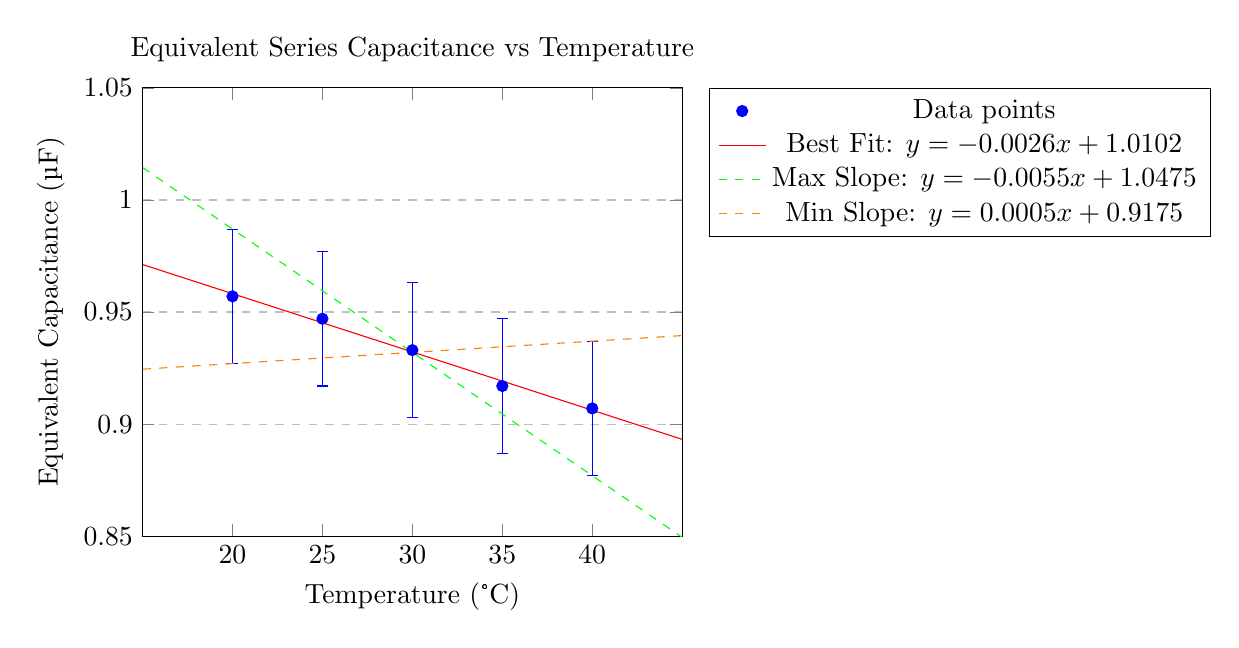
\begin{tikzpicture}
\begin{axis}[
    title={Equivalent Series Capacitance vs Temperature},
    xlabel={Temperature (°C)},
    ylabel={Equivalent Capacitance (µF)},
    xmin=15, xmax=45,
    ymin=0.85, ymax=1.05,
    xtick={20,25,30,35,40},
    ytick={0.85, 0.90, 0.95, 1.00, 1.05},
    legend style={at={(1.05,1)}, anchor=north west}, % This positions the legend outside to the right
    ymajorgrids=true,
    grid style=dashed,
    error bars/y dir=both,
    error bars/y explicit,
]

% Adding data points
\addplot[
    only marks,
    color=blue,
    mark=*,
    error bars/.cd,
    y dir=both, y explicit
    ]
    coordinates {
    (20,0.957) +- (0,0.03)
    (25,0.947) +- (0,0.03)
    (30,0.933) +- (0,0.03)
    (35,0.917) +- (0,0.03)
    (40,0.907) +- (0,0.03)
    };
\addlegendentry{Data points}

% Adding line of best fit
\addplot[
    domain=15:45,
    samples=100,
    color=red,
]
{-0.0026*x + 1.0102};
\addlegendentry{Best Fit: $y = -0.0026x + 1.0102$}

% Adding max and min slopes
\addplot[
    domain=15:45,
    samples=100,
    color=green,
    dashed,
]
{-0.0055*x + (0.957 + 0.03 - (-0.0055*20))};
\addlegendentry{Max Slope: $y = -0.0055x + 1.0475$}

\addplot[
    domain=15:45,
    samples=100,
    color=orange,
    dashed,
]
{0.0005*x + (0.957 - 0.03 - (0.0005*20))};
\addlegendentry{Min Slope: $y = 0.0005x + 0.9175$}

\end{axis}
\end{tikzpicture}
\caption{Plot of Equivalent Series Capacitance vs. Temperature with Line of Best Fit and Slope Uncertainty}
\end{figure}
\noindent Hence, this experiment aligns with the theoretical background, as the increase in temperature did correspond to a decrease in the capacitance of the capacitors in series across all 3 capacitors, suggesting a decrease in the ability of the capacitors to hold charge when subject to increased temperature changes. While the data was not strictly linear originally, performing the linear regression helped demonstrate a more direct relationship between the two quantities.\\
\noindent In conclusion, while the battery serves an important role in electronics, the "wear and tear" often discarded as natural and normal for systems is often a result of a lack of care and maintenance of components like capacitors, which are significantly affected by changes in temperature. This aligns with the aforementioned research. In electronics, temperature changes are frequent due to components like the CPU and graphical processing unit, leading to deviations in responses and a decrease in efficiency as demonstrated by this data.

\section{Evaluation}
\subsection{Limitations}
Components of the experiment caused some inaccuracies, most prominently the assumption that the wire's resistance was negligible. As a result of this assumption, at higher temperatures, where resistance increases due to increased collisions, the capacitance of the capacitor was affected as the current began to model that of an RC circuit, leading to increased inaccuracy and uncertainty at higher temperatures. I noticed this when measuring with my capacitance meter, as the time it took to stabilize was significantly higher, and the value continued to fluctuate even after, suggesting a non-negligible resistance. This effect is more pronounced after each trial as I did not replace the circuit after each trial, so prolonged exposure may have caused further resistance. Increased precision in measurement tools would have also helped with more precise analysis of the data, as well as uncertainty, as it is seemingly uniform and may not reveal much about the reliability of data trials in comparison to one another.
\subsection{Strengths}
However, the use of multiple trials and the evident trend established, combined with minimially flucuating values for the linear regressions, suggest that the linear regression overcomes this limitation. Another strength of the experiment is the effeciency of the experiment, as industrial-grade equipment was used (namely the water bath and stable direct current power supply) allowing for precise control of the independent variable, and improvements to the equipment regarding the measurements of the dependent variable would have amplified this effect. Furthermore, the use of distilled water and recyclable materials makes this experiment sustainable and minimizes any potential impacts.

\subsection{Further Exploration}
 For future research, one could utilize different mediums that might be commonplace within electronics and act as liquid dielectric when permeating them, such as impure water which acts as a suspender for dust and other particles (and consequently, acts as an ion carrier and is electrically conductive). Furthermore, a more complete circuit that can replicate the vast array of capacitors present in a phone could shed light on how such changes in capacitance actually affect the phones' processes, allowing for a better evaluation of the significance of this data and conclusion.

\printbibliography

\end{document}


